\chapter{Formal Model}
\label{ch:formal-model}

\textbf{Reader's Guide:} This chapter formalizes the concurrency control and
liveness properties of the proposed Software Transactional Memory (STM) system,
establishing the theoretical correctness on how the system handles opacity and global progress. The corresponding implementation is covered in
Chapter~\ref{ch:implementation}.

\section{Preliminaries}

To formally define the system, we abstract the state into two core
ideas: a timeline of global progress and the individual versioned variables.

Let $\mathcal{W}$ be the totally ordered set of \emph{write points}, where each
$w \in \mathcal{W}$ is a positive integer corresponding to a snapshot of the
global version clock. Let $\mathcal{R}$ be the set of \emph{transactional
references}, where each $r \in \mathcal{R}$ maintains a fixed
history of versioned values indexed by write points. Let $\mathcal{V}$ be the
set of all reference values.

Each reference $r \in \mathcal{R}$ is associated with a partial function
$\mathit{hist}(r) : \mathcal{W} \rightharpoonup \mathcal{V}$ that maps a write point to
the value committed at that point. For a transaction with read point $w_r$, the visible
value of $r$ is defined as:
\[
  \mathit{snap}(r,\, w_r)
    = \mathit{hist}(r)(w')
    \quad \text{where } w' = \max\bigl\{\, w \in \mathcal{W}
        \mid w \leq w_r,\; w \in \operatorname{dom}(\mathit{hist}(r)) \,\bigr\}
\]
That is, $\mathit{snap}$ returns the value committed at the latest write point that
(i)~does not exceed $w_r$ and (ii)~is in the domain of $\mathit{hist}(r)$, i.e.\ some
transaction actually wrote $r$ at that point.

\section{Transactions and Histories}

\begin{definition}[Transaction]
A transaction $T$ is a tuple $T = \langle\, id,\; w_r,\; RS,\; WS,\; \sigma
\,\rangle$ where:
\begin{itemize}
  \item $id \in \mathbb{N}$ is a unique monotonically increasing transaction
        identifier.
  \item $w_r \in \mathcal{W}$ is the \emph{read point}, the value of the
        global version clock at the time $T$ was created.
  \item $RS : \mathcal{R} \rightharpoonup \mathcal{W} \times \mathcal{V}$ is
        the \emph{read set}, mapping each reference read during $T$ to a tuple
        $e = (w, v)$ containing the write point and value observed.
  \item $WS : \mathcal{R} \rightharpoonup \mathcal{V}$ is the \emph{write set},
        mapping each reference to its speculative value.
  \item $\sigma \in \{\textsc{Active},\, \textsc{Aborted},\,
        \textsc{Committed}\}$ is the transaction status.
\end{itemize}
\end{definition}

\begin{definition}[History and Concurrency~{\cite{guerraoui2007,bushkov2012}}]
A \emph{history} $H$ of the system is a sequence of invocation and response
events produced by concurrent transactions. $H$ is \emph{well-formed} if for
every transaction $T$ in $H$, the events of $T$ form a sequence of alternating
invocations and responses.
\end{definition}

We consider only well-formed histories throughout. Following Bushkov et
al.~\cite{bushkov2012}, transaction $T$ is \emph{committed} if its last event
is a commit event and \emph{aborted} if its last event is an abort event.

\section{Operations}

Each transaction $T$ supports the following operations on references:

\paragraph{Read.} $\text{deref}(r)$ returns:
\[
  \text{deref}(r) =
  \begin{cases}
    WS[r]                  & \text{if } r \in \text{dom}(WS) \\
    RS[r].\mathit{value}   & \text{if } r \in \text{dom}(RS) \\
    \text{snap}(r,\; w_r)  & \text{otherwise}
  \end{cases}
\]

\paragraph{Write.}
$\text{ref-set}(r, v)$ requires $T$ to acquire ownership of $r$.
Let $\text{owner}(r) \in \mathbb{N} \cup \{ \bot \}$ denote the ID of the
transaction currently owning the speculative write for $r$.
Ownership is resolved as:
\[
\text{acquire}(T, r) =
\begin{cases}
    \text{True} & \text{if } \text{owner}(r) = \bot \lor \text{owner}(r) = T.id \\
    \text{True}, \sigma_{T'} \gets \textsc{Aborted} & \text{if } \text{owner}(r) = T'.id \land T'.id < T.id \\
    \text{Abort} & \text{if } \text{owner}(r) = T'.id \land T'.id > T.id
\end{cases}
\]
On success, $WS[r] \gets v$.

\section{Execution}

An \emph{execution} of transaction $T$ over function $f$ produces an outcome:
\[
  \text{execute}(T, f) =
  \begin{cases}
    \textsc{Ok}(v)
      & \text{if } f \text{ completes and } T \text{ commits successfully} \\
    \textsc{Abort}
      & \text{if an } \textsc{Aborted} \text{ signal is raised during } f \text{ or commit} \\
    \textsc{Exception}(e)
      & \text{if any other exception } e \text{ is raised}
  \end{cases}
\]

The transaction retry loop behaves as follows:
\[
\text{run-tx}(f, T) =
\begin{cases}
v
  & \text{if } \text{execute}(T,f)=\textsc{Ok}(v) \\[6pt]

\text{run-tx}(f, T')
  & \text{if } \text{execute}(T,f)=\textsc{Abort} \;\land\; T'=\text{next-tx}(T) \\[6pt]

\text{raise}(e)
  & \text{if } \text{execute}(T,f)=\textsc{Exception}(e)
\end{cases}
\]

where $\text{next-tx}(T)$ is a retry transition producing a new transaction with an incremented id, subject to retry limits.

\section{Commit Protocol}

A transaction $T$ with a non-empty write set ($\mathrm{dom}(WS) \neq \emptyset$) commits under a global commit lock. Upon entering the commit phase, the system checks $\sigma_T$. If $\sigma_T = \textsc{Aborted}$, the transaction is aborted and the commit is canceled.

If $T$ is still active, its read-set is validated against reference modifications by:
\[
\text{valid}(T) \triangleq \forall (r, e) \in RS:\;
\text{write-point}(r) \leq \text{write-point}(e)
\]

If $\text{valid}(T)$ does not hold, the transaction is aborted.

If validation succeeds, a new write point $w_c$ is allocated atomically. The transaction applies its writes to the global state and releases ownership of each written reference:
\[
    \text{owner}(r) \gets \bot \quad \forall\, r \in \mathrm{dom}(WS)
\]

Read-only transactions ($\mathrm{dom}(WS) = \emptyset$) skip the commit lock entirely, as their snapshot consistency is guaranteed by versioned reads.

\section{Safety: Opacity}

The correctness criterion of the proposed system is \emph{opacity}.
Intuitively, opacity guarantees that every transaction observes a logically consistent timeline, preventing crashes from unexpected states. Guerraoui and Kapalka~\cite{guerraoui2007} define opacity
through three requirements:
\begin{enumerate}
    \item \textbf{Atomicity:} Operations of committed transactions must appear
          to execute at a single indivisible point in time.
    \item \textbf{Isolation:} Operations of aborted transactions must never be
          visible to other transactions.
    \item \textbf{Consistency:} Every transaction must always observe a
          consistent system state, regardless of its final status.
\end{enumerate}

A \emph{completion} of a history $H$ is obtained by either appending a commit event or an
abort event to each transaction that has no final event in $H$, or by removing it
entirely. $\mathit{Complete}(H)$ denotes the set of all such completions~\cite{guerraoui2007}.

\begin{definition}[Opacity~{\cite{guerraoui2007}}]
A history $H$ is \emph{opaque} if there exists a sequential history $S$
equivalent to some history in $\text{Complete}(H)$, such that $S$ preserves
the real-time order of $H$ and every transaction $T_i \in S$ is \emph{legal}
in $S$.
\end{definition}

\begin{definition}[Legality~{\cite{guerraoui2007}}]
A transaction $T_j$ is \emph{legal} in a sequential history $S$ if, for every
reference $r$ read by $T_j$, the value observed is the value written by the
most recent committed transaction that wrote $r$ before $T_j$ in $S$, or the
initial value of $r$ if no such transaction exists.
\end{definition}

The key distinction from strict serializability is that opacity requires
legality for \emph{every} transaction in $S$, including aborted and live ones.
The proposed system guarantees opacity through two mechanisms:

\paragraph{Immutable Snapshots via $w_r$.}
Every transaction reads exclusively from the snapshot determined by its read
point $w_r$ via the $\text{snap}(r, w_r)$ function. Because these snapshots
are composed only of values from previously committed transactions, $T$ is
guaranteed to observe a state that was consistent at $w_r$.

\paragraph{Termination of Zombie Transactions.}
A status check before every critical operation ensures that no transaction
continues execution after its ownership has been stolen. This prevents zombie
transactions, those logically aborted but still physically executing,
from observing inconsistent states produced by concurrent writes after $w_r$.

Together, these properties ensure that every transaction observes only states
that could have arisen in a valid serial execution, satisfying opacity as
defined in~\cite{guerraoui2007}.

\begin{figure}[ht]
\centering
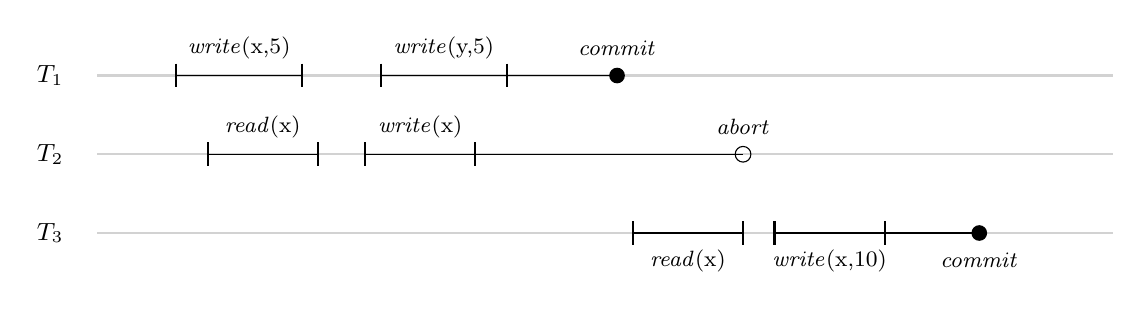
\begin{tikzpicture}[
  tx/.style={font=\small},
  op/.style={font=\footnotesize},
  line/.style={gray!35, thick},
  tick/.style={thick},
  commit/.style={circle, fill=black, inner sep=2pt},
  abort/.style={circle, draw, inner sep=2pt}
]
\node[tx] at (0,0)   {$T_1$};
\node[tx] at (0,-1)  {$T_2$};
\node[tx] at (0,-2)  {$T_3$};

\draw[line] (0.6,0) -- (13.5,0);
\draw[line] (0.6,-1) -- (13.5,-1);
\draw[line] (0.6,-2) -- (13.5,-2);

\draw (1.6,0) -- (3.2,0);
\draw[tick] (1.6,0.15)--(1.6,-0.15);
\draw[tick] (3.2,0.15)--(3.2,-0.15);
\node[op] at (2.4,0.35) {\textit{write}(x,5)};
\draw (4.2,0) -- (5.8,0);
\draw[tick] (4.2,0.15)--(4.2,-0.15);
\draw[tick] (5.8,0.15)--(5.8,-0.15);
\node[op] at (5.0,0.35) {\textit{write}(y,5)};
\draw (5.8,0) -- (7.2,0);
\node[commit] at (7.2,0) {};
\node[op] at (7.2,0.35) {\textit{commit}};

\draw (2.0,-1) -- (3.4,-1);
\draw[tick] (2.0,-0.85)--(2.0,-1.15);
\draw[tick] (3.4,-0.85)--(3.4,-1.15);
\node[op] at (2.7,-0.65) {\textit{read}(x)};
\draw (4.0,-1) -- (5.4,-1);
\draw[tick] (4.0,-0.85)--(4.0,-1.15);
\draw[tick] (5.4,-0.85)--(5.4,-1.15);
\node[op] at (4.7,-0.65) {\textit{write}(x)};
\draw (5.4,-1) -- (8.8,-1);
\node[abort] at (8.8,-1) {};
\node[op] at (8.8,-0.65) {\textit{abort}};

\draw (7.4,-2) -- (8.8,-2);
\draw[tick] (7.4,-1.85)--(7.4,-2.15);
\draw[tick] (8.8,-1.85)--(8.8,-2.15);
\node[op] at (8.1,-2.35) {\textit{read}(x)};
\draw (9.2,-2) -- (10.6,-2);
\draw[tick] (9.2,-1.85)--(9.2,-2.15);
\draw[tick] (10.6,-1.85)--(10.6,-2.15);
\node[op] at (9.9,-2.35) {\textit{write}(x,10)};
\draw (10.6,-2) -- (11.8,-2);
\node[commit] at (11.8,-2) {};
\node[op] at (11.8,-2.35) {\textit{commit}};
\end{tikzpicture}
\caption{An opaque history: $T_2$ is aborted but still observes a consistent
snapshot, satisfying the opacity requirement of~\cite{guerraoui2007}.}
\end{figure}

\section{Liveness: Impossibility of Local Progress and the Adopted Guarantee}

While safety ensures the system never returns an incorrect result, liveness
ensures the system makes forward progress under contention. A system that aborts
every transaction trivially satisfies opacity but makes no useful progress.
Formalising what progress a correct STM \emph{can} guarantee requires care, and
the theoretical bounds established by Bushkov and Guerraoui~\cite{bushkov2012}
directly shape the guarantees claimed here.

\paragraph{Starvation under adversarial scheduling.}
The impossibility of local progress manifests as \emph{starvation}. A
transaction $T_1$ that reads a reference $r$ may be indefinitely denied if a
succession of transactions $T_2, T_3, \ldots$ each write $r$ and commit before
$T_1$ can do so. Each such commit advances the write point of $r$ beyond $T_1$'s
read point, causing read-set validation to fail and forcing another retry. Under
adversarial scheduling this cycle repeats without bound. The proposed system does
not eliminate this possibility; doing so would contradict Theorem~1
of~\cite{bushkov2012}, since any mechanism guaranteeing $T_1$'s eventual commit
would require blocking concurrent writers, which is incompatible with opacity.

\begin{figure}[ht]
\centering
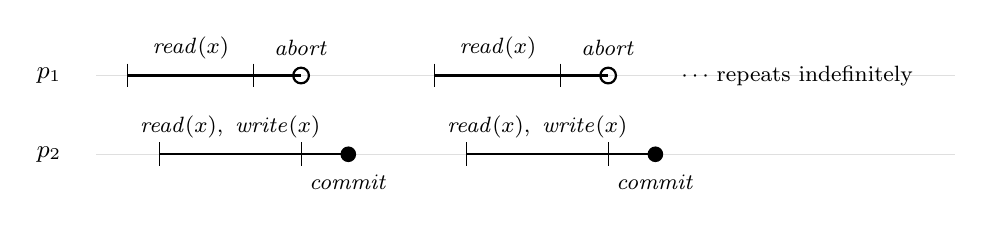
\begin{tikzpicture}[
  tx/.style={font=\small},
  op/.style={font=\footnotesize},
  tline/.style={thick},
  commit/.style={circle, fill=black, inner sep=2pt},
  abort/.style={circle, draw, thick, inner sep=2pt},
]
\node[tx] at (0, 0)  {$p_1$};
\node[tx] at (0, -1) {$p_2$};
\draw[gray!25] (0.6, 0) -- (11.5, 0);
\draw[gray!25] (0.6, -1) -- (11.5, -1);

\draw[tline] (1.0, 0) -- (2.6, 0);
\draw (1.0,0.15)--(1.0,-0.15); \draw (2.6,0.15)--(2.6,-0.15);
\node[op] at (1.8,0.35) {$\mathit{read}(x)$};
\draw[tline] (1.4, -1) -- (3.2, -1);
\draw (1.4,-0.85)--(1.4,-1.15); \draw (3.2,-0.85)--(3.2,-1.15);
\node[op] at (2.3,-0.65) {$\mathit{read}(x),\ \mathit{write}(x)$};
\draw[tline] (3.2,-1) -- (3.8,-1);
\node[commit] at (3.8,-1) {};
\node[op] at (3.8,-1.35) {\textit{commit}};
\draw[tline] (2.6,0) -- (3.2,0);
\node[abort] at (3.2,0) {};
\node[op] at (3.2,0.35) {\textit{abort}};

\draw[tline] (4.9, 0) -- (6.5, 0);
\draw (4.9,0.15)--(4.9,-0.15); \draw (6.5,0.15)--(6.5,-0.15);
\node[op] at (5.7,0.35) {$\mathit{read}(x)$};
\draw[tline] (5.3,-1) -- (7.1,-1);
\draw (5.3,-0.85)--(5.3,-1.15); \draw (7.1,-0.85)--(7.1,-1.15);
\node[op] at (6.2,-0.65) {$\mathit{read}(x),\ \mathit{write}(x)$};
\draw[tline] (7.1,-1) -- (7.7,-1);
\node[commit] at (7.7,-1) {};
\node[op] at (7.7,-1.35) {\textit{commit}};
\draw[tline] (6.5,0) -- (7.1,0);
\node[abort] at (7.1,0) {};
\node[op] at (7.1,0.35) {\textit{abort}};

\node[op] at (9.5, 0) {$\cdots$ repeats indefinitely};
\end{tikzpicture}
\caption{Starvation scenario: $p_2$ repeatedly commits before $p_1$, forcing
$p_1$ to abort forever.}
\end{figure}

\paragraph{Parasitic transactions.}
Bushkov et al.~\cite{bushkov2012} define a \emph{parasitic} process as one that
executes transactional operations indefinitely without ever invoking a commit
request. Such a process loops without committing but is repeatedly displaced by
newer transactions via ownership stealing, ensuring it never prevents progress
while its speculative state never reaches the committed history of any reference.

\begin{figure}[ht]
\centering
\begin{tikzpicture}[
  tx/.style={font=\small},
  op/.style={font=\footnotesize},
  line/.style={gray!25, thick},
  tline/.style={thick},
  commit/.style={circle, fill=black, inner sep=2pt},
  stolen/.style={circle, draw=red, thick, inner sep=2pt},
]
\node[tx] at (0, 0)    {$T_p$};
\node[tx] at (0, -1.8) {$T_n$};

\draw[line] (0.6, 0)    -- (10.5, 0);
\draw[line] (0.6, -1.8) -- (10.5, -1.8);

\draw[tline] (0.8,0) -- (1.6,0);
\draw (0.8,0.15)--(0.8,-0.15);
\draw (1.6,0.15)--(1.6,-0.15);
\node[op] at (1.2,0.38) {$r(x)$};

\draw[tline] (1.6,0) -- (2.4,0);
\draw (2.4,0.15)--(2.4,-0.15);
\node[op] at (2.0,0.38) {$r(x)$};

\draw[tline] (2.4,0) -- (3.4,0);
\draw (3.4,0.15)--(3.4,-0.15);
\node[op] at (2.9,0.38) {$w(x)$};

\node[stolen] at (3.8,0) {};
\node[op,red] at (3.8,0.38) {\textit{stolen}};

\draw[-{Stealth}, thick, dashed, gray]
  (3.8,-0.2) .. controls (4.6,-0.8) and (0.4,-0.8) .. (0.8,-0.15);
\node[op,gray] at (2.3,-0.88) {loops (never commits)};

\draw[tline] (3.0,-1.8) -- (4.2,-1.8);
\draw (3.0,-1.65)--(3.0,-1.95);
\draw (4.2,-1.65)--(4.2,-1.95);
\node[op] at (3.6,-1.45) {$w(x)$};
\draw[tline] (4.2,-1.8) -- (5.0,-1.8);
\node[commit] at (5.0,-1.8) {};
\node[op] at (5.0,-2.15) {\textit{commit}};
\end{tikzpicture}
\caption{A parasitic transaction $T_p$ loops indefinitely. A newer transaction
$T_n$ steals ownership (marked \textcolor{red}{\textit{stolen}}), aborting
$T_p$ and committing successfully. $T_p$ loops back and never reaches a commit,
but never blocks $T_n$ either.}
\end{figure}

\paragraph{Executions and outcomes.}
A single transaction attempt returns one of three outcomes:
$\textsc{Ok}(v)$ if the transaction committed successfully;
$\textsc{Abort}$ if the transaction was invalidated by a failed read-set check
or by ownership being stolen; or $\textsc{Exception}(e)$ if an unexpected error
propagated. The retry loop retries on $\textsc{Abort}$ and re-throws on
$\textsc{Exception}(e)$. If the retry count reaches a fixed maximum, the system
throws unconditionally rather than retrying indefinitely.

A \emph{history} $H$ of the system is the sequence of outcome events produced
by all threads over an execution. For a thread $p_k$ we write $H|_{p_k}$ for
the projection of $H$ onto the outcomes of that thread.

\paragraph{Process classifications.}
Following Bushkov and Guerraoui~\cite{bushkov2012}, threads are partitioned into
classes according to their observable behaviour in a history.

\begin{definition}[Correct Process~{\cite{bushkov2012}}]
A thread $p_k$ is \emph{correct} in $H$ if $H|_{p_k}$ contains infinitely many
$\textsc{Ok}(v)$ or $\textsc{Abort}$ outcomes: that is, $p_k$ persists
indefinitely without exiting via $\textsc{Exception}(e)$.
\end{definition}

\begin{definition}[Crashed Process~{\cite{bushkov2012}}]
A thread $p_k$ is \emph{crashed} in $H$ if $H|_{p_k}$ is finite. The history
is augmented with a crash event $\mathit{crash}^k$ immediately after the last
outcome of $p_k$.
\end{definition}

\begin{definition}[Parasitic Process~{\cite{bushkov2012}}]
A thread $p_k$ is \emph{parasitic} in $H$ if $H|_{p_k}$ contains infinitely
many outcomes but only $\textsc{Abort}$ outcomes from some point onward, with no
intervening $\textsc{Ok}(v)$, due to the thread never reaching the commit phase.
\end{definition}

\paragraph{Progress.}
A correct thread $p_k$ \emph{makes progress} in $H$ if $H|_{p_k}$ contains
infinitely many $\textsc{Ok}(v)$ outcomes. A thread producing only
$\textsc{Abort}$ outcomes indefinitely is \emph{starved}.

\paragraph{Local progress and its impossibility.}

\begin{definition}[Local Progress~{\cite{bushkov2012}}]
A history $H$ ensures \emph{local progress} if every correct thread makes
progress:
\[
  H \text{ ensures local progress} \;\iff\;
  \forall\, p_k \in \mathit{Correct}(H) :\;
  |\{\,\textsc{Ok}(v) \in H|_{p_k}\}| = \infty
\]
\end{definition}

Theorem~1 of Bushkov and Guerraoui~\cite{bushkov2012} establishes that no TM
implementation can ensure both opacity and local progress in a fault-prone
system. The proposed system does not claim local progress; doing so would
require blocking concurrent writers, which is incompatible with opacity.

\paragraph{Global progress as the adopted guarantee.}

\begin{definition}[Global Progress~{\cite{bushkov2012}}]
A history $H$ ensures \emph{global progress} if at least one correct thread
makes progress:
\[
  H \text{ ensures global progress} \;\iff\;
  \exists\, p_k \in \mathit{Correct}(H) :\;
  |\{\,\textsc{Ok}(v) \in H|_{p_k}\}| = \infty
\]
\end{definition}

Global progress is strictly weaker than local progress and is compatible with
opacity~\cite{bushkov2012}.

\begin{theorem}[Deadlock Freedom and Global Progress]
Let $\prec$ be the total strict ordering on transactions defined by
$T_i \prec T_j \iff T_i.id < T_j.id$. The ownership-resolution policy
guarantees that the implementation is deadlock-free and ensures global
progress in the sense of~\cite{bushkov2012}.
\end{theorem}

\begin{proof}
Since $id$ is assigned from a global monotonically increasing atomic counter,
$\prec$ forms a strict total order over all created transactions. Ownership of
a reference $r$ is granted to $T_j$ over $T_i$ if and only if $T_i \prec T_j$.
Because a transaction can only be preempted by one strictly greater in $\prec$,
cyclic dependencies are impossible, establishing deadlock freedom.

In any non-empty set of competing transactions, there exists $T_{max}$ such that
$\forall T_i \neq T_{max}: T_i \prec T_{max}$. $T_{max}$ successfully acquires
all required ownerships without being aborted. It then enters the commit phase,
where read-set validation ensures its snapshot remains consistent. Thus in every
contention round at least one correct process is guaranteed to commit,
satisfying global progress.
\end{proof}

\paragraph{Termination under absence of contention.}
A transaction $T$ that encounters no conflicting concurrent writes commits on
its first attempt. The validation condition is trivially satisfied when no other
transaction has written to any ref in $RS$ since $w_r$.

\paragraph{Progress under contention via ownership stealing.}
When two transactions $T_i$ and $T_j$ compete for the same reference, the one
with the strictly greater identifier is granted ownership:
\[
  \text{owner}(r) \gets T_j.id \quad \text{if } T_j.id > T_i.id,\quad
  \sigma_{T_i} \gets \textsc{Aborted}
\]
This guarantees at least one winner per contention round. It is, however, the
same mechanism responsible for starvation: a transaction repeatedly preempted by
newer ones may never obtain ownership long enough to commit. This is precisely
the trade-off admitted by~\cite{bushkov2012}: global progress is achievable but
local progress is not.

\paragraph{Bounded backoff.}
When a transaction is aborted and retried, exponential backoff with jitter is applied
after the fourth retry. The delay grows with the retry count up to a fixed cap of
$32\,\text{ms}$, with $\pm 25\%$ random jitter to prevent the thundering-herd problem.
Because the cap is finite, worst-case per-retry latency is bounded regardless of
contention level. The precise formula is given in Section~\ref{sec:retry}.